\begin{table}[H]
    \centering
    \caption{DTW Results Comparison} \label{tb:dtw_com}
    \begin{tabular}{lrr}
    \toprule
    Metric & Benchmark Value & Model Value\\
    \midrule
    DTW Distance & 63 2& 23.0 \\  % The total cost (distance) of aligning your two sequences
    Normalized DTW Distance & 0.0815 & 0.0029 \\  % DTW distance normalized by the length of the alignment path
    Alignment Path Length & 15,464 & 15,464 \\
    Diagonal Ratio & 1.996 & 1.995 \\   % 	Measures deviation from perfect 1-to-1 alignment. Closer to 1 = better
    \bottomrule
    \end{tabular}
\end{table}

\begin{table}[H]
    \centering
    \caption{Wasserstein Distance Results Comparison}
    \label{tb:wasserstein_com}
    \begin{tabular}{lrr}
    \toprule
    Metric & Benchmark Value & Model Value\\
    \midrule
    Wasserstein Distance & 0.1054 & 0.0019 \\  % The average time difference between predicted and actual events.
    Normalized Distance & 0.1054 & 0.0019 \\  % 10.54% of the worst-case possible mismatch
    Maximum Possible Distance & 1.0000 & 1.0000 \\
    \bottomrule
    \end{tabular}
\end{table}

\begin{table}[H]
    \centering
    \caption{Allan Factor Results Comparison}
    \label{tb:allan-factor_com}
    \begin{tabular}{lccc}
    \toprule
    \textbf{Window Size} & $\bar{\alpha}_\text{true}$ & $\bar{\alpha}_\text{pred}$ & $\bar{\alpha}_\text{benchmark}$ \\
    \midrule
    2   & 1.044 & 0.869 & 0.452 \\
    5   & 1.044 & 1.290 & 1.148 \\
    10  & 0.958 & 1.159 & 2.303 \\
    20  & 1.090 & 1.346 & 4.582 \\
    50  & 1.050 & 1.722 & 9.064 \\
    \midrule
    \textbf{Average AF} & 1.0698 & 1.2687 & 4.9571 \\
    \textbf{Number of Events} & 23 & 38 & 840 \\
    \textbf{Event Rate} & 0.00297 & 0.00490 & 0.108387 \\
    \bottomrule
    \end{tabular}
\end{table}

\begin{table}[H]
    \centering
    \begin{tabular}{lccc}
    \toprule
    \textbf{Metric} & $\bar{\alpha}_\text{true}$ & $\bar{\alpha}_\text{pred}$ & $\bar{\alpha}_\text{benchmark}$ \\
    \midrule
    Number of Events & 23 & 38 & 840 \\
    Event Intensity (events/sec) & 0.0128 & 0.0211 & 0.4667 \\
    Average \( L(r) \) & 22.7610 & 31.04 & 48.3360 \\
    \( L(1s) \) & 12.6101 & 13.96 & 17.4891\\
    \( L(2s) \) & 11.6101 & 15.45 & 25.2693\\
    \( L(5s) \) & 15.4251 & 22.42 & 39.4575\\
    \bottomrule
    \end{tabular}
    \caption{Ripley's L Function Comparison for true, predicted, and benchmark aggressive trade indicators}    
    \label{tb:ripley-l_com}
\end{table}


\begin{table}[htbp]
\centering
\begin{tabular}{lccc}
\toprule
\textbf{Metric} & $\bar{\alpha}_{\text{true}}$ & $\bar{\alpha}_{\text{pred}}$ & $\bar{\alpha}_{\text{benchmark}}$ \\
\midrule
Lag-1 autocorrelation       & 0.0842  & 0.1310  & 0.7196  \\
Lag-5 autocorrelation       & -0.0030 & 0.0224  & 0.3897  \\
Lag-10 autocorrelation      & -0.0030 & -0.0048 & 0.2428  \\
\# Significant lags         & 6       & 14      & 48      \\
Has significant autocorr    & True    & True    & True    \\
\bottomrule
\end{tabular}
\caption{Autocorrelation comparison for true, predicted, and benchmark aggressive trade indicators}
\label{tab:acf-series-com}
\end{table}

\begin{figure}[H]
    \centering
    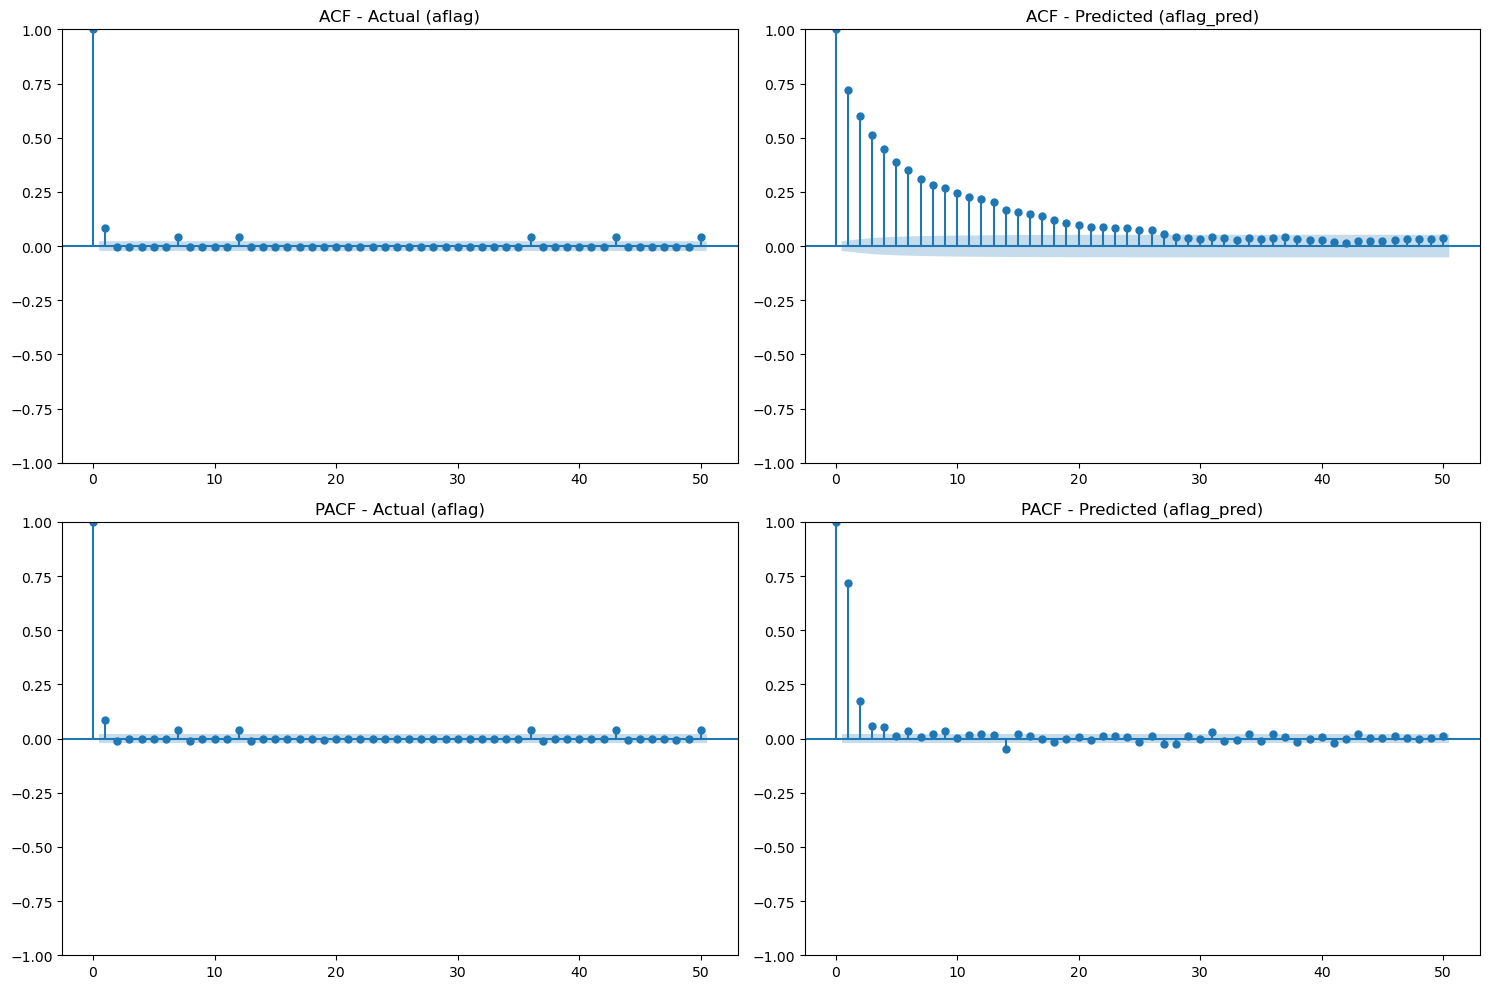
\includegraphics[width=0.95\linewidth]{figures/ACF_181330_benchmark.png}
    \caption{Autocorrelation (ACF) and Partial Autocorrelation (PACF) plots of actual and benchmark predicted aggressive trade series.}
    \label{fig:acf-pacf-com}
\end{figure}


\begin{table}[H]
    \centering
    \caption{Kolmogorov--Smirnov Test Results Comparison}
    \label{tb:ks-test-com}
    \begin{tabular}{lrr}
    \toprule
    \textbf{Metric} & \textbf{Benchmark Value} & \textbf{Model Value}\\
    \midrule
    KS Statistic & 0.1054 & 0.0019 \\
    p-value & 0.000 & 1.0000 \\
    Significant ($p < 0.05$) & True & False \\
    Actual Proportion & 0.0030 & 0.0030 \\
    Predicted Proportion & 0.1084 & 0.0049 \\
    Proportion Difference & 0.1054 & 0.0019 \\
    \bottomrule
    \end{tabular}
\end{table}

